\section{Zahnräder}
\subsection{Stirnräder}
\subsubsection{Breiten-/ Durchmesserverhältnisse:}
Formeln aus dem Skript zur Konstruktionslehre III\ccite{bib:poll:kl3} Seiten 150 - 153:
\begin{align*}
&b \cdot d^2 \ge\frac{2 \cdot M}{B_{zul}} \\
&\frac{b}{d} = (0,1...0,5) + \frac{i}{20} \\
&d \ge \sqrt[3]{\frac{2 \cdot M}{( \frac{b}{d}) \cdot  4 \frac{\text{N}}{\text{mm}^2}}}
\end{align*}
\begin{itemize}
\item {Z\textsubscript{1}/Z\textsubscript{2}/Z\textsubscript{3}:}
\begin{align*}
	& \left(\frac{b}{d} \right) _{1,2} = (0,1...0,5) + \frac{i_{1,2}}{20} \text{ mit } i_{1,2} = i_{1,3}= 3 \\
	&\left(\frac{b}{d} \right) _{1,2}= \left(\frac{b}{d} \right) _{1,3} = (0,25...0,65) \\
	&d_1 \ge \sqrt[3]{\frac{2 \cdot 95290 \text{ Nmm}}{(0,25...0,65) \cdot  4 \frac{\text{N}}{\text{mm}^2}}}= (41,85...57,55) \text{ mm}\\
	&d_2 \ge \sqrt[3]{\frac{2 \cdot 71470 \text{ Nmm}}{(0,25...0,65) \cdot  4 \frac{\text{N}}{\text{mm}^2}}}= (38,02...52,29) \text{ mm}  \\
	&d_3 \ge \sqrt[3]{\frac{2 \cdot 285870 \text{ Nmm}}{(0,25...0,65) \cdot  4 \frac{\text{N}}{\text{mm}^2}}}= (60,36...83) \text{ mm}\\
	&b_1= \left(\frac{b}{d} \right) _{1,2}  \cdot d_1 = (10,46...37,4) \text{ mm}  \\
	&b_2= \left(\frac{b}{d} \right) _{1,2}  \cdot d_2 = (9,5...33,99) \text{ mm}  \\
	&b_3= \left(\frac{b}{d} \right) _{1,3}  \cdot d_3 = (15,09...53,95) \text{ mm}  
\end{align*}
\item {Z\textsubscript{4}/Z\textsubscript{5}:}
\begin{align*}
	& \left(\frac{b}{d} \right) _{4,5} = (0,1...0,5) + \frac{i_{4,5}}{20} \text{ mit } i_{4,5} =  3,77 \\
	&\left(\frac{b}{d} \right) _{4,5}=  (0,29...0,69) \\
	&d_4 \ge \sqrt[3]{\frac{2 \cdot 71470 \text{ Nmm}}{(0,29...0,69) \cdot  4 \frac{\text{N}}{\text{mm}^2}}}= (37,29...49,82) \text{ mm}\\
	&d_5 \ge \sqrt[3]{\frac{2 \cdot 268990 \text{ Nmm}}{(0,29...0,69) \cdot  4 \frac{\text{N}}{\text{mm}^2}}}= (58...77,5) \text{ mm}  \\
	&b_4= \left(\frac{b}{d} \right) _{4,5}  \cdot d_4 = (10,78...34,33) \text{ mm}  \\
	&b_5= \left(\frac{b}{d} \right) _{4,5}  \cdot d_5 = (16,76...53,4) \text{ mm}  
\end{align*}
\item {Z\textsubscript{6}/Z\textsubscript{7}:}
\begin{align*}
	& \left(\frac{b}{d} \right) _{6,7} = (0,1...0,5) + \frac{i_{6,7}}{20} \text{ mit } i_{6,7} =  1,89 \\
	&\left(\frac{b}{d} \right) _{6,7}=  (0,19...0,59) \\
	&d_6 \ge \sqrt[3]{\frac{2 \cdot 285870 \text{ Nmm}}{(0,19...0,59) \cdot  4 \frac{\text{N}}{\text{mm}^2}}}= (62,37...90,95) \text{ mm}\\
	&d_7 \ge \sqrt[3]{\frac{2 \cdot 268990 \text{ Nmm}}{(0,19...0,59) \cdot  4 \frac{\text{N}}{\text{mm}^2}}}= (61,09...89,12) \text{ mm}  \\
	&b_6= \left(\frac{b}{d} \right) _{6,7}  \cdot d_6 = (11,84...53,66) \text{ mm}  \\
	&b_7= \left(\frac{b}{d} \right) _{6,7}  \cdot d_7 = (11,61...52,58) \text{ mm}  
\end{align*}
\end{itemize}
\subsubsection{Profilverschiebung Z4/Z5:}
Formeln zur Berechnung der Profilverschiebung aus Roloff/Matek\ccite{bib:roloffMatek:maschinenelemente} S. 786-791 und S. 789-800 :
\begin{align*}
\text{Teilkreisdurchmesser: }&d = z \x \frac{m_n}{\cos(\beta)} \\
\text{Wälzkreisdurchmesser: }&d_w = d \x \frac{\cos(\alpha_t)}{\cos(\alpha_{\omega t})} \\
\text{Grundkreisdurchmesser: }&d_b = d \x \cos(\alpha_t) \\
\text{Fußkreisdurchmesser: }&d_f = d -2 \x ((m+c)-V)\\
\text{Kopfrücknahme: }&k = \Delta a -m_n \x (x_1+x_2)\\
\text{Kopfkreisdurchmesser: }&d_a = d +2 \x (m_n+V +k)\\
\text{Aufteilung Profilverschiebung: }& x_1 \approx \frac{x_1 + x_2}{2} + \left( 0,5 - \frac{x_1+x_2}{2} \right) \x \frac{\lg(u)}{\lg\left( \frac{z_1 \x z_2}{100} \right)} \\
\text{Ersatzzähnezahl: }& z_n = \frac{z}{\cos^3\beta} \\
\text{Profilverschiebung: }& V = x \x m_n 
\end{align*}
\begin{itemize}
\item Vorauslegung:
\begin{align*}
	&a= 215 \text{ mm, } \alpha = \beta = 20^\circ \\
	&\left. \begin{array}{c} a= \frac{d_4 + d_5}{2}\\i_{4,5} = \frac{d_5}{d_4} \end{array} \right\} \text{ }d_4 = \frac{2 \x a}{1+i_{4,5}} \\
	&d_4 = \frac{2\x 215 \text{ mm}}{1+3,77} = 90,15\text{ mm} \\
	&d_5 = d_4 \x i_{4,5} = 339,87 \text{ mm}\\
	&\text{Wähle: }m_n = 4 \text{ mm} \\
	&z_4 = \frac{90,15 \text{ mm} \x \cos(20^\circ)}{4 } \text{ mm} = 21,18 \implies z_4 = 21\\
	&z_5 = \frac{339,87 \text{ mm} \x \cos(20^\circ)}{4 } \text{ mm} = 79,84 \implies z_5 = 80 \\
	&\implies d_4 = \frac{21 \x 4\text{ mm} }{\cos(20^\circ)} = 89,39093 \text{ mm} \\
	&\implies d_5 = \frac{80\x 4\text{ mm} }{\cos(20^\circ)} = 340,53689 \text{ mm} \\
	&a* = 214,96391 \text{ mm} 
\end{align*}
\item Modul und Eingriffswinkel:
\begin{align*}
	&m_t = \frac{m_n}{\cos(\beta)} = 4,257\text{ mm} \\
	&\text{Eingriffswinkel Teilkreis: } \alpha_t = \tan^{(-1)} \left( \frac{\tan(\alpha)}{\cos(\beta)} \right) = 21,17283 ^\circ \\
	&\text{Eingriffswinkel Wälzkreis: } \alpha_{\omega t} = \arccos \left( \frac{a*}{a} \x \cos(\alpha_t)\right) = 21,19765 ^\circ \\
	&inv(\alpha) = \tan(\alpha) -\alpha \x \frac{\pi}{180^\circ} \\
	&inv(\alpha_t) = 0,017793 \\
	&inv(\alpha_{\omega t}) = 0,017858 
\end{align*}
\item Profilverschiebungsfaktoren:
\begin{align*}
	&x_4 + x_5 = \frac{inv(\alpha_{\omega t})-inv(\alpha_{t})}{2 \x \tan(\alpha_{n})} \x (z_4 + z_5) = \frac{a - a*}{m_n} = 0,009 \\
	&z_{n,4} = \frac{21}{\cos^3(20^\circ)} = 25,3 \text{ , }z_{n,5} = \frac{80}{\cos^3(20^\circ)} = 96,41 \\
	&x_4 =\frac{0,009}{2} + \left( 0,5 - \frac{0,009}{2} \right) \x \frac{\lg(3,77)}{\lg\left( \frac{21 \x 80}{100} \right)} = 0,238 \\
	&x_5 = 0,009 - 0,238 = - 0,229 \\ 
	&V_4 = 0,238 \x 4 \text{ mm} = 0,953 \text{ mm, }V_5 = -0,229\x 4 \text{ mm} = -0,916 \text{ mm} 
\end{align*}
\newpage
\item Graphische Bestimmung der Profilverschiebungsfaktoren und Ersatzzähnezahlen:
\begin{center}
	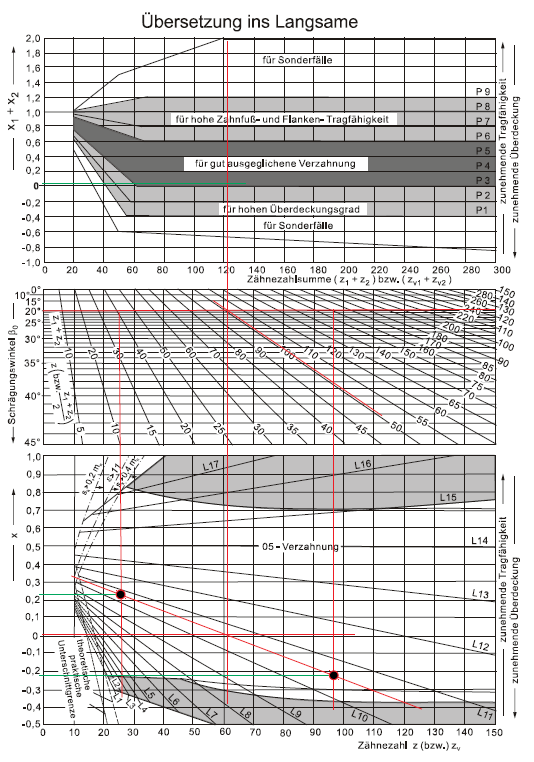
\includegraphics[width=0.95\textwidth,keepaspectratio]{figures/Profilverschiebung45.png}
\end{center}
Aus der graphischen Kennzeichnung sind folgende Werte abzulesen:
\begin{align*}
	&x_4 \approx 0,23 &x_5 \approx -0,22 \\
	&z_{n,4} \approx 25 & z_{n,5} \approx 96	
\end{align*}
Die graphisch ermittelten Werte der Zahnradstufe 4/5 stimmen ungefähr mit den berechneten überein. \\
\item endgültige Werte:
\begin{align*}
	&z_4 = 21 \text{ , } z_5 = 80 \\
	&d_4 = 89,39 \text{ mm} \\
	&d_{w,4} = 89,39  \text{ mm}\x \frac{\cos(21,17283^\circ)}{\cos(21,19765^\circ)} = 89,41  \text{ mm}\\
	&d_{b,4} = 89,39  \text{ mm} \x \cos(21,17283^\circ) = 83,36  \text{ mm}\\
	&d_{f,4} = 89,39  \text{ mm} -2 \x ((4,257 \text{ mm}+1,06)-0,953) = 80,66 \text{ mm}\\
	&k_4 = -0,039 \text{ mm} -4 \text{ mm} \x (0,009) =- 0,051 \text{ mm}\\
	&d_{a,4} = 89,39  \text{ mm} +2 \x (4\text{ mm}+0,953 \text{ mm} -0,051 \text{ mm}) = 99,2\text{ mm}\\
	&d_5 =340,54 \text{ mm} \\
	&d_{w,5} = 340,54  \text{ mm}\x \frac{\cos(21,17283^\circ)}{\cos(21,19765^\circ)} = 340,6  \text{ mm}\\
	&d_{b,5} = 340,54  \text{ mm} \x \cos(21,17283^\circ) = 317,55  \text{ mm}\\
	&d_{f,5} = 340,54  \text{ mm} -2 \x ((4,257 \text{ mm}+1,06)+0,916) = 328,1 \text{ mm}\\
	&k_5 = -0,039 \text{ mm} -4 \text{ mm} \x (0,009) =- 0,051 \text{ mm}\\
	&d_{a,5} = 340,54  \text{ mm} +2 \x (4\text{ mm}-0,916 \text{ mm} -0,051 \text{ mm}) = 346,6\text{ mm}
\end{align*}
\end{itemize}
\subsubsection{Profilverschiebung Z6/Z7:}
\begin{itemize}
\item Vorauslegung:
\begin{align*}
	&a= 215 \text{ mm, } \alpha = \beta = 20^\circ \\
	&\left. \begin{array}{c} a= \frac{d_6 + d_7}{2}\\i_{6,7} = \frac{d_7}{d_6} \end{array} \right\} \text{ }d_6 = \frac{2 \x a}{1+i_{6,7}} \\
	&d_6 = \frac{2\x 215 \text{ mm}}{1+1,89} = 148,79\text{ mm} \\
	&d_7 = d_6 \x i_{6,7} = 281,21 \text{ mm}\\
	&\text{Wähle: }m_n = 4 \text{ mm} \\
	&z_6 = \frac{148,79 \text{ mm} \x \cos(20^\circ)}{4 } \text{ mm} = 34,95 \implies z_6 = 35\\
	&z_7 = \frac{281,21 \text{ mm} \x \cos(20^\circ)}{4 } \text{ mm} = 66,06 \implies z_7 = 66 \\
	&\implies d_6 = \frac{35 \x 4\text{ mm} }{\cos(20^\circ)} = 148,98489 \text{ mm} \\
	&\implies d_7 = \frac{66\x 4\text{ mm} }{\cos(20^\circ)} = 280,942932\text{ mm} \\
	&a* = 214,96391 \text{ mm} 
\end{align*}
\item Modul und Eingriffswinkel:
\begin{align*}
	&m_t = \frac{m_n}{\cos(\beta)} = 4,257\text{ mm} \\
	&\text{Eingriffswinkel Teilkreis: } \alpha_t = \tan^(-1) \left( \frac{\tan(\alpha)}{\cos(\beta)} \right) = 21,17283 ^\circ \\
	&\text{Eingriffswinkel Wälzkreis: } \alpha_{\omega t} = \arccos \left( \frac{a*}{a} \x \cos(\alpha_t)\right) = 21,19765 ^\circ \\
	&inv(\alpha) = \tan(\alpha) -\alpha \x \frac{\pi}{180^\circ} \\
	&inv(\alpha_t) = 0,017793 \\
	&inv(\alpha_{\omega t}) = 0,017858 
\end{align*}
\item Profilverschiebungsfaktoren:
\begin{align*}
	&x_6 + x_7 = \frac{inv(\alpha_{\omega t})-inv(\alpha_{t})}{2 \x \tan(\alpha_n)} \x (z_6 + z_7) = \frac{a - a*}{m_n} = 0,009 \\
	&z_{n,6} = \frac{35}{\cos^3(20^\circ)} = 42,18 \text{ , }z_{n,7} = \frac{66}{\cos^3(20^\circ)} = 79,54 \\
	&x_6 =\frac{0,009}{2} + \left( 0,5 - \frac{0,009}{2} \right) \x \frac{\lg(1,89)}{\lg\left( \frac{35 \x 66}{100} \right)} = 0,105 \\
	&x_7 = 0,009 - 0,105 = - 0,096 \\ 
	&V_6 = 0,105 \x 4 \text{ mm} = 0,42 \text{ mm, }V_7 = -0,096\x 4 \text{ mm} = -0,384 \text{ mm} 
	\end{align*}
\newpage
\item Graphische Bestimmung der Profilverschiebungsfaktoren und Ersatzzähnezahlen:
	\begin{center}
		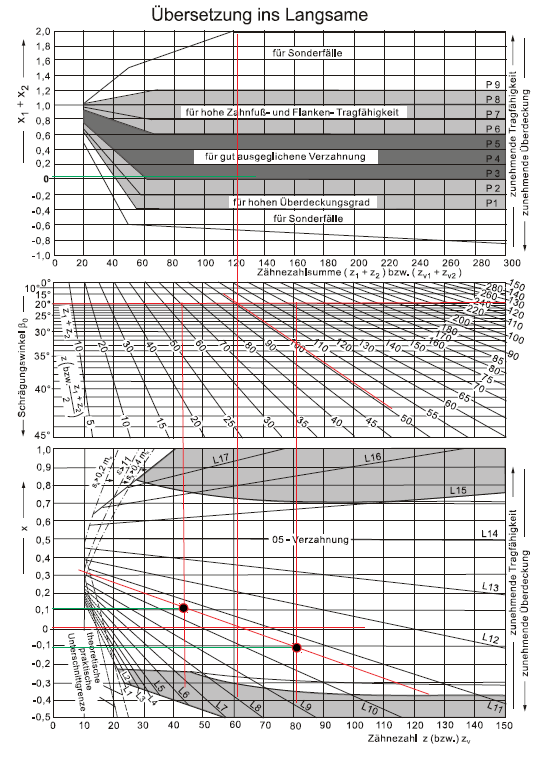
\includegraphics[width=0.95\textwidth,keepaspectratio]{figures/Profilverschiebung67.png}
	\end{center}
Aus der graphischen Kennzeichnung sind folgende Werte abzulesen:
\begin{align*}
	&x_6 \approx 0,105 &x_7 \approx -0,105 \\
	&z_{n,6} \approx 43 & z_{n,7} \approx 81	
\end{align*}
Die graphisch ermittelten Werte stimmen ungefähr mit den berechneten überein. Die Werte von Zahnrad 7 weisen leichte Abweichungen auf, was an Ungenauigkeiten in der Zeichnung liegt. \\
\item endgültige Werte:
\begin{align*}
	&z_6 = 35 \text{ , } z_7 = 66 \\
	&d_6 = 148,98 \text{ mm} \\
	&d_{w,6} = 148,98  \text{ mm}\x \frac{\cos(21,17283^\circ)}{\cos(21,19765^\circ)} = 149 \text{ mm}\\
	&d_{b,6} = 148,98  \text{ mm} \x \cos(21,17283^\circ) = 138,9  \text{ mm}\\
	&d_{f,6} = 148,98  \text{ mm} -2 \x ((4,257 \text{ mm}+1,06)-0,42) = 139,19 \text{ mm}\\
	&k_6 = -0,039 \text{ mm} -4 \text{ mm} \x (0,009) =- 0,051 \text{ mm}\\
	&d_{a,6} = 148,98  \text{ mm} +2 \x (4\text{ mm}+0,42 \text{ mm} -0,051 \text{ mm}) = 157,72\text{ mm}\\
	&d_7 =280,94 \text{ mm} \\
	&d_{w,7} =280,94  \text{ mm}\x \frac{\cos(21,17283^\circ)}{\cos(21,19765^\circ)} = 280,99  \text{ mm}\\
	&d_{b,7} = 280,94  \text{ mm} \x \cos(21,17283^\circ) = 261,98 \text{ mm}\\
	&d_{f,7} = 280,94  \text{ mm} -2 \x ((4,257 \text{ mm}+1,06)+0,384) = 269,54 \text{ mm}\\
	&k_7 = -0,039 \text{ mm} -4 \text{ mm} \x (0,009) =- 0,051 \text{ mm}\\
	&d_{a,7} = 280,94  \text{ mm} +2 \x (4\text{ mm}-0,384 \text{ mm} -0,051 \text{ mm}) = 288,1\text{ mm}
\end{align*}	
\end{itemize}
\newpage
\subsubsection{Erste Getriebestufe:}
Die verwendeten Formeln stammen aus dem Roloff/Matek\ccite{bib:roloffMatek:maschinenelemente} Seite 796:
\begin{align*}
	&d= z \x \frac{m_n}{\cos(\beta)} \\
	&d_a = m_n \cdot (\frac{z}{\cos(\alpha_n)}+2)\text{, } d_f =d- 2,5 \x m_n
\end{align*}
\begin{align*}
	&\text{Wähle: } m_n= 4\text{ mm, } d_2 = d_3 = 210 \text{ mm} \\
	&m_t =  \frac{m_n}{\cos(\beta)} = 4,26 \text{ mm} \\
	&d_1 = \frac{d_3}{i_{1,3}} = 70 \text{ mm} \\
	&z_1 = \frac{70 \text{ mm} \x \cos(20^\circ)}{4 \text{ mm}} \text{ mm} = 16,4 \implies z_1 = 17\\
	&z_2=z_3 = z_1 \x i_{1,3} =19 \x 3 = 51 \\
	&d_{1,neu} = \frac{17 \x 4 \text{ mm}}{\cos(20^\circ)} = 72,36 \text{ mm} \\
	&d_{2,neu} = d_{3,neu} = \frac{51 \x 4 \text{ mm}}{\cos(20^\circ)} = 217,1 \text{ mm} \\
	&d_{1,a} = 4\text{ mm} \x \left(\frac{17}{\cos(20^\circ)}+2\right) =80,36\text{ mm} \\
	&d_{1,f} = 72,36\text{ mm} -2,5 \x 4\text{ mm} =62,36\text{ mm} \\
	&d_{2,a} = d_{3,a} =4\text{ mm} \x \left(\frac{51}{\cos(20^\circ)}+2\right) =225,09\text{ mm} \\
	&d_{2,f} =d_{3,f} = 217,1\text{ mm} -2,5 \x 4\text{ mm} =207,1\text{ mm} 
\end{align*}
\subsection{Planetengetriebe}
Um das Planetengetriebe auszulegen, werden zunächst die Einzelübersetzungen ermittelt (siehe Roloff/Matek\ccite{bib:roloffMatek:maschinenelemente} Seite 884). Anschließend wird der Mindestdurchmesser des Sonnenrades (Z8) bestimmt. Damit lassen sich dann durch Übersetzungsverhältnisse die Durchmesser der Planetenräder bestimmen. 
\newpage
Die verwendeten Formeln für Fuß- und Kopfkreisdurchmesser stammen aus dem Roloff/Matek\ccite{bib:roloffMatek:maschinenelemente} S. 780: $d_a = m_n \x (z + 2) \text{, } d_f = m_n \x (z-2,5) $
\begin{align*}
	&\text{Wähle } m=4  \text{ mm} \\
	&i_{8,9} = 1 - i_0 = 4 \\
	&i_{9,8} = \frac{1}{1-i_0}  = 0,25 \\
	& \left(\frac{b}{d} \right) _{9,8} = (0,1...0,5) + \frac{0,25}{20}  =  (0,11...0,51) 
\end{align*}
\begin{itemize}
\item Sonnenrad
\begin{align*}
	&d_8 \ge \sqrt[3]{\frac{2 \cdot 71470 \text{ Nmm}}{(0,11...0,51) \cdot  4 \frac{\text{N}}{\text{mm}^2}}}= (41,23...68,74) \text{ mm}\\
	&b_8= \left(\frac{b}{d} \right) _{9,8}  \cdot d_8 = (4,54...35,1) \text{ mm}  \\
	&\text{wähle: } d_8 = 112 \text{ mm, } b_8 = 35 \text{ mm}  \\
	&z_8 = \frac{d_8}{m} = 28 \\
	&d_{8,a} = 4\text{ mm} \x (28+2) =120\text{ mm} \\
	&d_{8,f} = 4\text{ mm} \x (28-2,5) =102\text{ mm} 
\end{align*}
\item Planetenräder 
\begin{align*}
	&d_9 = \frac{i_{8,9} \x d_8}{2 } - d_8 = 112 \text{ mm}  \\
	&z_9 = \frac{d_9}{m} = 28 \\
	&\text{wähle }  b_9 = 28 \text{ mm}  \\
	&d_{9,a} = 4\text{ mm} \x (28+2) =120\text{ mm} \\
	&d_{9,f} = 4\text{ mm} \x (28-2,5) =102\text{ mm} \\ 
	&\text{Anzahl Planeten: } \frac{z_{8} + z_{10}}{4} = 32,25 \implies 4 \text{ Planeten} 
\end{align*}	
\item Hohlrad:
\begin{align*}
	&d_{10} = d_8 + 2\x d_9 = 336 \text{ mm}  \\
	&\text{wähle }  b_{10} = 30 \text{ mm}  \\
	&z_{10}  = \frac{d_{10}}{m} = 84 \\
	&d_{10,f} = 4\text{ mm} \x (84+2,5) =346\text{ mm} \\
	&d_{10,f} = 4\text{ mm} \x (84-2) =328\text{ mm} 
\end{align*}	
\end{itemize}
\subsection{Kegelräder}
Die Abmaße der Kegelräder werden mit den Formeln aus Roloff/Matek\ccite{bib:roloffMatek:maschinenelemente} Seite 832 bis 835 ermittelt. Dabei werden zunächst Richtwerte ermittelt, auf deren Basis dann die endgültigen Abmaße bestimmt werden.
\begin{align*}
	&\text{Achsenwinkel } \sum = \delta_{11} + \delta_{12} = 90^\circ \\
	&\delta_{11}= \delta_{12} =  45^\circ \text{ , da die Übersetzung } i_{11,12} =1
\end{align*}
Nach Tabelle 22-1 aus Roloff/Matek Tabellenbuch\ccite{bib:roloffMatek:tabellenbuch}: $z_{11} = z_{12} = 30$ \\
\textbf{mittlerer Modul:}\\
aus Roloff/Matek\ccite{bib:roloffMatek:maschinenelemente} Seite 841
\begin{align*}
	&m'_m \ge \frac{\left(2,4...2,6\right) \cdot d_{sh}}{z} \\
	&m'_m \ge \frac{\left(2,4...2,6\right) \cdot d_{\mathrm{IV}}}{z_{11}} = \frac{\left(2,4...2,6\right) \cdot 40\text{ mm}}{30} = (3,2...3,5) \text{mm} 
\end{align*}
\textbf{Breitenverhältnis:}
\begin{align*}
	&\frac{b}{d} = \frac{\left((0,1...0,5)+ \frac{i}{10}\right) \cdot i}{\sqrt{i^2 + 1}} \text{ mit } i_{11,12} = 1 \\
	&\frac{b}{d} = (0,14...0,42) \\
	&\left. \begin{array}{c} F_t \ge B_{zul} \cdot d \cdot b\\T = \frac{d}{2} \cdot F_t \end{array} \right\} \text{ }b \cdot d^2 \ge \frac{2 \cdot T}{B_{zul}} 
\end{align*}
\[
\implies d^3 \ge \frac{2 \cdot T}{(0,19...0,51) \cdot B_{zul}} \text{ mit } T_{\mathrm{IV}} = 268,99 \text{ Nm und  } B_{zul} = 4 \frac{\text{N}}{\text{mm}^2}
\]
\begin{align*}
	&d_{11} \ge \sqrt[3]{\frac{2 \cdot 268990 \text{ Nmm}}{(0,14...0,42) \cdot  4 \frac{\text{N}}{\text{mm}^2}}}= (68,42...98,67) \text{ mm} \\
	&b_{11} = (68,42 \cdot 0,14 ...98,67 \cdot 0,42) \text{ mm} = (9,58...41,44) \text{ mm}
\end{align*}
\textbf{äußerer Teilkreisdurchmesser:}
\[
d_{e,min} = d_{m,min} + b_{min}\cdot\sin\delta_{11} = 68,42 \text{ mm} + 9,58 \text{ mm} \cdot \sin 45^\circ =75,2 \text{ mm}
\]
\[
d_{e,max} = d_{m,max} + b_{max}\cdot\sin\delta_{11} =98,67 \text{ mm} + 41,44 \text{ mm} \cdot \sin 45^\circ =128 \text{ mm}
\]
\textbf{äußere Teilkegellänge:}
\[
R_{e,min} = \frac{d_{e,min}}{2 \cdot \sin \delta_{11}} = 53,17 \text{ mm}
\]
\[
R_{e,max} = \frac{d_{e,max}}{2 \cdot \sin \delta_{11}} = 90,5 \text{ mm}
\]

\textbf{äußerer Modul:}
\[
m_e = \frac{d_e}{z_{11}} = \frac{(75,2...128)}{30} = (2,5...4,3) \text{ mm}
\]
\textbf{endgültige Abmaße:}
\begin{align*}
	&b= 28 \text{ mm} \\
	&m_e=4 \text{ mm} \\ 
	&d_{e,11} =d_{e,12} = z_{11} \cdot m_e = 30 \cdot 4 \text{ mm} = 120 \text{ mm} \\
	&R_e \ge 3 \cdot b = 84 \text{ mm} \\
	&R_e = \frac{d_{e,11}}{2 \cdot \sin \delta_{11}} = 84,85 \text{ mm}
\end{align*}
\begin{itemize}
	\item Zahnkopf-, Zahnfuß-, und Zahnhöhe:
	\[
	h_{ae} = m_e = 4 \text{ mm; } h_{fe} = 1,25 \cdot m_e =5 \text{ mm; } h_e = 2,25 \cdot m_e = 9 \text{ mm}
	\]
	\item äußerer Kopfkreisdurchmesser:
	\[
	d_{ae,11} = m_e \cdot (z_{11} + 2 \cdot \cos \delta_{11}) = 125,66 \text{ mm}
	\]
	\[
	d_{ae,12} = m_e \cdot (z_{12} + 2 \cdot \cos \delta_{12}) = 125,66 \text{ mm}
	\]
\end{itemize}